\chapter{Mesh and Collider creation}

\section{Mesh Generation}
The maze generation algorithms discussed operate on the classes \texttt{Maze}, \texttt{MazeCell} and \texttt{MazeWall}. However these classes are merely the representation of a mathematical model. In order to use this maze in a 3D environment we need to convert these elements into a 3D mesh. This process is called {\em procedural modelling}. The procedural modelling is carried out by the \texttt{BasicMeshMaker} class with the help of the \texttt{VertexFactory} class. The class creates an array of \texttt{MazeMesh} instances.

\subsection{Procedural modelling}
Procedural modelling is a very difficult task because it essentially involves writing a program that will simulate the human behaviour of a 3D graphics artist. Fortunately, man-made structures such as mazes generally follow a pattern that can be exploited in the modelling process. For instance: walls are designed to be nothing more than a basic cuboid, although detail can always be added to make them look less like a cuboid. Like with many other man-made structures, the floor of the dungeon is intended to be a flat plane.

In order to start procedural modelling, we first need to understand how the 3D plane primitive works because this will be used extensively throughout the algorithm. The plane primitive is composed of 4 corners and 2 triangles (or 1 quad depending on the rendering mode chosen). Divisions can also be added across the plane to increase the polygon count although this is not always necessary.

\begin{figure}[h!]
\centering
 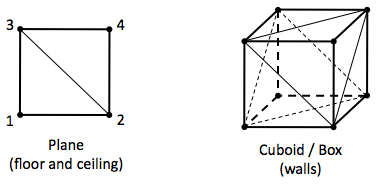
\includegraphics[width=0.52\textwidth]{images/what_is_a_plane.png}
\caption{Vertices and edges of the 3D meshes used to procedurally model the dungeon.}
\end{figure}

The plane can be used as the floor and ceiling of the dungeon to provide a satisfying result. However the plane primitive cannot be used for the walls because this will evidently cause the walls to look far too thin. Therefore we need to use the box primitive for the wall. The box is simply 6 planes stuck to one another.

\subsection{UVW mapping}
Defining the vertex position is not sufficient to produce a good result. In order to render a texture onto the walls and the floor of the dungeon we need to apply a material with a diffuse texture onto those meshes. Each vertex of those meshes will also require a texture coordinate so that the graphics shader can sample the texture for each 3D primitive face.

The question is: how do we define these texture coordinates? Obviously, these coordinates are dependent on the shape of the meshes. For the floor, which we can assume is just a plane, this UVW mapping is very simple to calculate because we can simply map each corner of the plane to its respective corner of the texture. Example: the top-left vertex would map to the UV $(0,0)$, the bottom-right vertex would map to the UV $(1,1)$ and so on.

Using this method will cause the original image to be stretched or squashed if the dimension ratios of the plane and the image don't match. This can be avoided by {\em tiling} the image across the maze cells. Thus we need only to use a square tile texture and maps the corners of the plane to the UV coordinates $(0,0)$ and $(W,L)$, where $W$, and $L$ are width and length of the maze respectively.

For the wall, the procedural UVW mapping is slightly more complicated, although it can be kept simple if we assume that the texture used can be tiled. Because the maps are simply six planes, we can map one face to the texture just like with the floor. However, the face on the opposite side of these coordinates need to be {\em mirrored} so that when two walls are stuck together they will appear as a single wall with a contiguous texture.

\subsection{Adding prefabs}
If we only use planes and boxes to procedurally model our dungeon then the final result will feel very monotonous. This is because we are reusing the exact same shape and texture every time. To reduce the amount of repetition in the dungeon we can add some human-modelled meshes to it to give it more life.

In this project, OBJ files can be imported into the application. However, in order to keep the framework generic, we must not restrain the generator to only using OBJ files. So to keep the framework generic, the generator will simply work with file-names and not the actual mesh. The generator will have no idea what the mesh looks like but will assume that it is scaled, positioned and rotated correctly. Meshes will be placed relative to the walls of the dungeon, so the OBJ files must match these walls. The generator will assume that meshes are facing the front of the scene, scaled to match 1 unit as the length and height of a wall, and positioned such that point $(0,0,0)$ is the centre of the wall's base.

File-names are read from a database and each item is assigned a weight. This weight will allow the user to control the probability of placing specific meshes. Hence, the probability of picking a given item $i$ is:

$$ P(i) = \frac{w_i}{\sum\limits_{j=0}^{n} {w_j} } $$

Where $w_k$ is the weight of the item $k$ and $n$ is the total number of items.

\paragraph{Adding prefabs on the walls}
To decorate the dungeon with assets we can add props such as paintings on the walls. The algorithm that does this simply rolls a dice for each face of each wall (Of course, this ignores the faces that are in-accessible from any part of the dungeon). If the dice roll is above a specified threshold called the {\em density} then a random prefab is selected from the database using the weights to determine their respective probabilities. The use of this {\em density} variable allows the user to control the amount of props that are placed in the dungeon. The dice roll and density are values between 0 and 1. A density of 0 means that no prefabs will be placed at all, 1 means that a prefab will placed on every face. Therefore a density of 0.5 for example will create a dungeon that has prefabs on approximately half of the faces.

\paragraph{Adding doors}
In order to increase the realism of the dungeon it's a good idea to consider adding doors too. To position the doors we need to turn a wall into a door, but we cannot simply place the doors anywhere we want because this might not give a realistic result. There are constraints to consider. For example: placing a door in the middle of an empty space (i.e. no walls around the door) will look pathetic. Doors intuitively lead from one room to another or from a corridor to a room. The constraints that are checked to find potential door candidates are the following:
\begin{itemize}
\item {\bf Only consider walls that don't exist:} This constraint is used to avoid breaking the wall of an inaccessible cell, because this would cause the door to lead to a single-cell (i.e. a dead-end).
\item {\bf Insure the walls on the sides of the door exist:} If the door doesn't have walls on the sides then the players can simply walk around them. This type of door is particularly useless and should be avoided.
\item {\bf The door must lead to atleast one room:} As discussed, doors intuitively lead to a room. A room can be considered as any empty space of minimum size 2x2. Needless to say, this room should be adjacent to the door.
\end{itemize}

Other than checking for these specific constraints, the process of placing doors is identical to that of placing items on the walls themselves. Adding these prefab models to the dungeon greatly enhances the overall aesthetic of it. Unfortunately, if the library of prefabs used is not sufficiently large then many objects will reappear repeatedly. Therefore a very large library is required in order for this method to be efficient.








\section{Colliders used}
The interactions between the player and the dungeon are often very game-specific, thus we cannot generalise this. However, collision detection and response is a feature that is probably common amongst all 3D video games. Therefore this aspect is more or less compulsory to implement in a generic framework.

To test if one mesh $M_1$ is colliding with another mesh $M_2$, the perfect collision detection algorithm checks if any triangle of $M_1$ is colliding with any triangle of $M_2$. Although computers are fast, this brute-force method will quickly get very expensive for high-polygon meshes and as the number of meshes in the scene increases \citep{BVH}. In a real-time applications, this method is not acceptable and either an optimisation or an approximation must be used.

A typical form of optimisation is to use a bounding volume to test for collision detection. This consists of using a primitive shape such as a sphere or a box to approximate the area of mesh. Because of the mathematical simplicity of these primitives we can perform collision tests very quickly with a complexity of $\bigo{1}$ \citep{BVH}. Some common bounding volumes include the following:
\begin{itemize}
\item {\bf Bounding Sphere:} This consists simply of a {\em radius} and {\em centre}. This is the cheapest type of bounding volume but is generally quite in-accurate.
\item {\bf Axis-Aligned Bounding Box (AABB):} This is cuboid with a {\em width}, {\em length} and {\em height} (or simply a {\em volume}) along with its {\em centre}. The box always remains aligned with the $xyz$-axes of the world space.
\item {\bf Oriented Bounding Box (OBB):} Like the AABB, the OBB also has a volume and centre. However, it also has an {\em orientation} component, making it more accurate but also more expensive.
\item {\bf Bounding Frustum:} This bounding volume is typically used in frustum culling to check if an object is in the view-port of the camera.
\end{itemize}

We need to construct a bounding volume for each individual wall. In the dungeon, the walls are all aligned with the $xyz$-axes and are all box-like shapes. This makes the AABB an ideal candidate because it will provide very fast and extremely accurate results. For this reason the AABB volume will be exploited to the fullest potential. Nevertheless, this will restraint the dungeon to only being allowed to rotate 90\degree, although this is not a deal big because an AABB can be considered as an OBB with an orientation of 0\degree on each axis. Therefore extending the framework to support orientation would not be complicated.

To calculate the AABB we can use variables defined in the \texttt{Maze} class. To calculate the centre of the box we need the cell width $W$ and length $L$, the height of the wall $H$ and the indices $(i_x, i_z)$ of the wall:
\begin{itemize}
\item {\bf For vertical walls:} $(x,\,y,\,z)= (i_{x}W,\, \frac{H}{2},\, i_{z}L+\frac{L}{2})$
\item {\bf For horizontal walls:} $(x,\,y,\,z)= (i_{x}W+\frac{W}{2},\, \frac{H}{2} ,\, i_{z}L)$
\end{itemize}
To calculate the volumes, we can use the values of $W$, $L$ and $H$ directly along with the thickness of the walls $T$:
\begin{itemize}
\item {\bf For vertical walls:} $(w,\,h,\,l)= (T,\, H,\, L)$
\item {\bf For horizontal walls:} $(w,\,h,\,l)= (W,\, H,\, T)$
\end{itemize}

\subsection{Bounding Volume Hierarchy}
Despite the fact that bounding boxes are very time-efficient they remain very expensive once the mesh count in the scene is high. If the scene is composed of millions of bounding boxes then the testing phase will require a significant amount of time and drop the frame rate to an unacceptable level \citep{BVH}. The number of AABBs contained in our maze is of order $\bigo{xz}$ where $(x,z)$ is the dimension of the maze, and in the worst case where $x=z$ we get a quadratic complexity $\bigo{x^2}$. For example, a maze of dimension $(100,100)$ will have upto $20 000$ boxes. Therefore, an extra optimisation is absolutely mandatory in order for the framework to support applications that require a large scale maze.

\subsubsection{Theory}
One very efficient method to test for collisions amongst a large set of colliders is to use a Bounding Volume Hierarchy (BVH). The idea behind the BVH is to categorise the colliders into groups and sub-groups to quickly identify which colliders could be potentially colliding and which ones are definitely not colliding. The BVH structure divides the colliders in the form of a tree. The brute method of testing for collision with each individual collider has a complexity $\bigo{n}$, where $n$ is the total number of colliders. The BVH aims at turning this linear complexity into a logarithmic one: $\bigo{\log_{k}n}$ where $k$ is the number of children per parent node in the tree \citep{BVH}. 

All the leaf nodes are the colliders themselves that are used to determine whether a collision is occurring or not. Whereas the parent node contains a collider that encapsulates all of its children. When checking the collisions the upper nodes in the tree are tested first starting with the root. If a parent collides then the algorithm recursively checks the children. However if a parent doesn't collide then the children do not need to be tested, thus eliminating a large number of tests and speeding up the collision detection \citep{BVH}.

\subsubsection{Dividing the maze}
To construct a BVH for the maze that contains the colliders of the walls and the floor we can recursively divide the maze into four sections (top-left, top-right, bottom-left, bottom-right) until we reach the individual maze cells.

\begin{figure}[h!]
\centering
 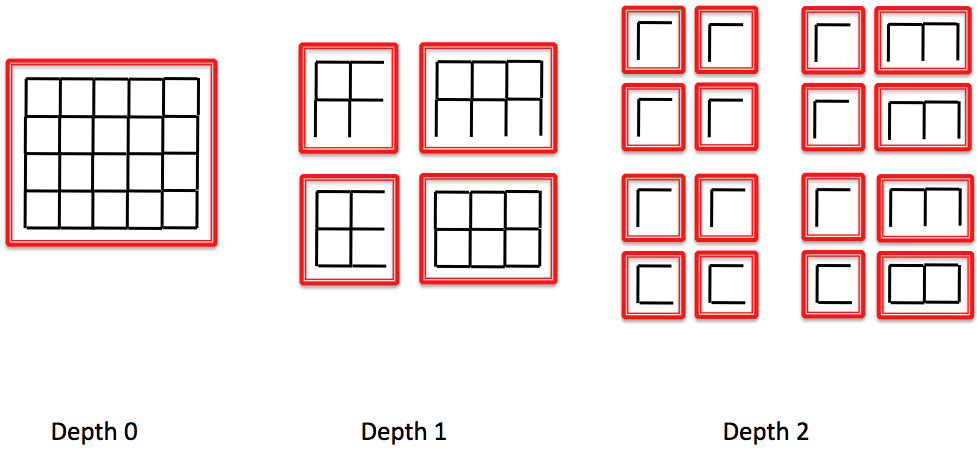
\includegraphics[width=0.74\textwidth]{images/bvh_maze.png}
\caption{An example of a BVH for a maze of dimension (5, 4). The red boxes represent parent nodes at a specific depth of the tree. The black lines represent the colliders of the walls.}
\end{figure}

However there are a few things to keep in mind:
\begin{enumerate}
\item {\bf The walls are shared amongst cells:} Although $k=4$ is used to sub-divide the maze we should avoid having the same collider stored twice in the BVH because this is an un-necessary waste of time and space. Therefore, when we reach the deepest parent nodes we should only have 2 children nodes: one for the top wall and another for the left wall.
\item {\bf There are more walls on the edge:} If we use the convention mentioned above then this would exclude all the walls on the very right and bottom edge of the maze. The nodes on those borders will need to have 3 or 4 children instead of 2.
\item {\bf Odd number division:} If a dimension is odd, then the bottom or right sections should be made slightly bigger to absorb the division's remainder and avoid colliders from getting excluded.
\end{enumerate}

The algorithm for constructing this BVH is given by:

\pagebreak
\lstAlgo
\begin{lstlisting}
func ConstructBVH(Maze M)
	Let C0 = cell number (0,0).
	Let C1 = cell number (M.Width-1, M.Length-1).
	Let R = ConstructNode(M, C0, C1).
	return a new BVH with root R.
endfunc

func ConstructNode(Maze M, Cell From, Cell To) // recursive
	Let R = a new BVH node.

	if From == To then
		Let L = Empty set {}.
		Calculate colliders of top and left walls. Add those to L.
		if To.X == Width-1  then add right wall to L as well. endif
		if To.Y == Height-1 then add bottom wall to L as well. endif
		Make L the children of R.
	else
		// Divide From-To into 4 spaces:
        /**
         *   +----+----+
         *   | S1 | S2 |
         *   +----+----+
         *   | S3 | S4 |
         *   +----+----+
         */
         foreach Non-empty space S in {S1, S2, S3, S4} do
         	Let C = ConstructNode(M, S.From, S.To).
         	Make C and child of R.
         endfor
	endif
	
	Calculate Bounding-box of R.
	return R.
endfunc
\end{lstlisting}